\section{DESCRIPCIÓN DE LA PRUEBA}
\begin{frame}{DESCRIPCIÓN DE LA PRUEBA}
\begin{itemize}
    \item La idea es determinar si hay diferencias significativas entre las medias de las poblaciones, comparando sus varianzas. Este método es una generalización de la \textit{prueba-t} de dos muestras, estudiado en clase \footnote{\bibentry{stat}}.
    \item Sea $k$ el número de poblaciones a ser analizadas, donde $Y_{ij}$ es la j-ésima unidad experimental para la i-ésima muestra, donde $i=1,...,k$ y $j=1,...,n_i$, donde $n_i$ es el tamaño de la i-ésima muestra.
    \item \textbf{Suposiciones:} Si el tamaño de la muestra es pequeño (i.e $n<30$), se debe suponer que la población sigue una distribución normal. Además, se supone que las poblaciones son independientes (tanto en muestras grandes como pequeñas) con medias $\mu_1,\mu_2,...,\mu_k$ y varianzas $\sigma_1^2=\sigma_2^2=...=\sigma_k^2=\sigma^2$.
    
    %La idea es hallar un estimador insesgado para $\sigma$.
\end{itemize}
\end{frame}
\subsection{Prueba de hipótesis}
\begin{frame}{DESCRIPCIÓN DE LA PRUEBA}
    \framesubtitle{Prueba de hipótesis}
    Basados en las pruebas ya mostradas, se requiere construir una prueba de hipótesis para determinar si existe evidencia suficiente para afirmar que $\mu_1=\mu_2=...=\mu_k$\footnote{\bibentry{stat}}.\vspace{2mm}
    
    \textbf{Hipótesis nula\\}
    $H_0:\quad\mu_1=\mu_2=...=\mu_k$
    \vspace{2mm}
    
    \textbf{Hipótesis alterna\\}
    $H_1:\quad(\exists\hspace{1mm} i,j)(\mu_i\ne\mu_j)\rightarrow$ Si al menos una de las igualdades no se cumple.\vspace{2mm}
    
    \begin{multicols}{2}
    \textbf{Estadístico de prueba\\}
    \[F=\dfrac{SST\Big/k-1}{SSE\Big/n-k}\sim\mathbb{F}_{(k-1,n-k)}\quad\text{, bajo } H_0\]
    \textbf{Región de Rechazo}
        \[RR:\left\{F>F_\alpha\right\}\]
        \columnbreak
        \begin{figure}[H]
            \centering
            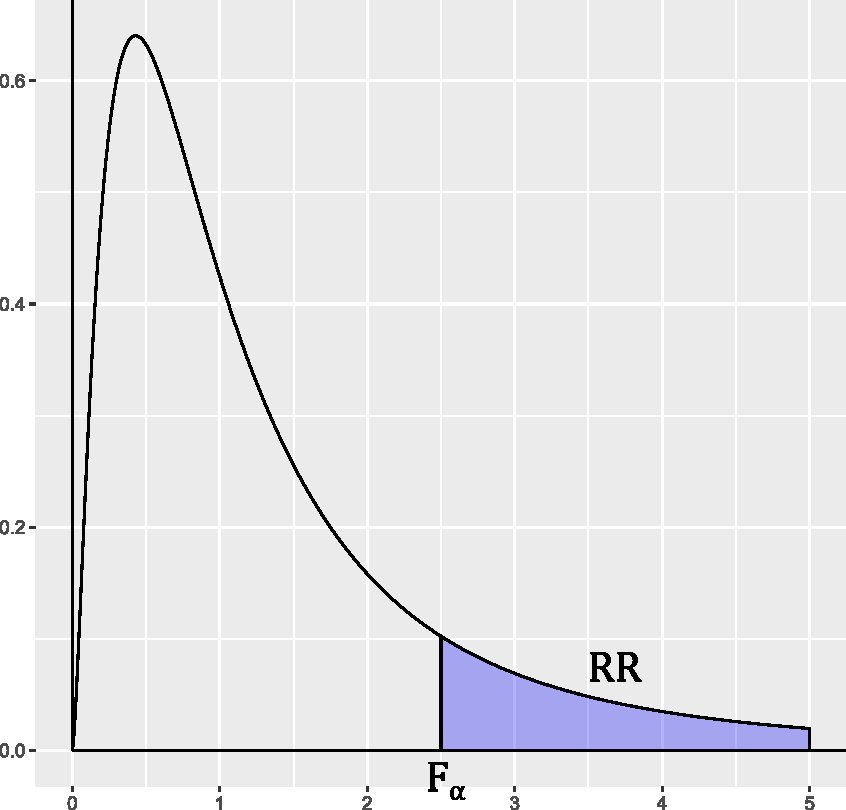
\includegraphics[width=45mm, height=35mm]{F.pdf}
        \end{figure}
    \end{multicols}
\end{frame}
\subsection{Preliminares}
\begin{frame}{DESCRIPCIÓN DE LA PRUEBA}
\framesubtitle{Preliminares}

    \begin{equation*}
        Y_i=\sum_{j=1}^{n_i}Y_{ij} \qquad E\left(Y_i\right)=n_i\mu_i \qquad V\left(Y_i\right)=n_i\sigma^2
    \end{equation*}
    \begin{equation*}
        \Bar{Y_i}=\dfrac{1}{n_i}Y_i \qquad E\left(\Bar{Y_i}\right)=\mu_i \qquad V\left(\Bar{Y_i}\right)=\dfrac{\sigma^2}{n_i}
    \end{equation*}
    \begin{equation*}
        \Bar{Y}=\dfrac{1}{n}\sum_{i=1}^kn_i\Bar{Y}_i\qquad\text{SST}=\sum_{i=1}^{k}\dfrac{Y_i^2}{n_i}-n\Bar{Y}^2\qquad \text{SSE}=\sum_{i=1}^{k}\sum_{j=1}^{n_i}\left(Y_{ij}-\Bar{Y}_i\right)^2
    \end{equation*}
    Se utilizarán estas variables aleatorias, con sus respectivas medias y varianzas, para calcular la esperanza del SST\footnote{\bibentry{stat}} (Total sum of squares), utilizando
    \begin{equation*}
        E\left(Y^2\right)=V(Y)+E^2\left(Y\right)
    \end{equation*}
        
    
\end{frame}

\begin{frame}{DESCRIPCIÓN DE LA PRUEBA}
\framesubtitle{Preliminares}
\begin{equation*}
\begin{split}
    E(SST)&=E\left(\sum_{i=1}^k\dfrac{Y_i^2}{n_i}\right)-E(n\Bar{Y}^2)\\
    &=\sum_{i=1}^k\dfrac{E\left(Y_i^2\right)}{n_i}-nE(\Bar{Y}^2)\\
    &=\sum_{i=1}^k\dfrac{n_i\sigma^2+(n_i\mu_i)^2}{n_i}-n\left(\dfrac{\sigma^2}{n}+\dfrac{1}{n^2}\left(\sum_{i=1}^kn_i\mu_i\right)^2\right)\\
    &=\sum_{i=1}^k\left(\sigma^2+n_i\mu_i^2\right)-\sigma^2-\dfrac{1}{n}\left(\sum_{i=1}^kn_i\mu_i\right)^2\\
    &=(k-1)\sigma^2+\sum_{i=1}^kn_i\mu_i^2-\dfrac{1}{n}\left(\sum_{i=1}^kn_i\mu_i\right)^2
\end{split}
\end{equation*}
\end{frame}

\begin{frame}{DESCRIPCIÓN DE LA PRUEBA}
\framesubtitle{Preliminares}
En el caso de $\mu_1=\mu_2=...=\mu_k=\mu$\footnote{\bibentry{stat}}, 
\begin{equation*}
    \begin{split}
        E(SST)&=(k-1)\sigma^2+\sum_{i=1}^kn_i\mu^2-\dfrac{1}{n}\left(\sum_{i=1}^kn_i\mu\right)^2\\
        &=(k-1)\sigma^2+\mu^2\sum_{i=1}^kn_i-\dfrac{\mu^2}{n}\left(\sum_{i=1}^kn_i\right)^2\\
        &=(k-1)\sigma^2+n\mu^2-n\mu^2
    \end{split}
\end{equation*}
    \begin{equation}
        E\left(\dfrac{SST}{k-1}\right)=\sigma^2
    \end{equation}
    Nótese que $\dfrac{SST}{k-1}$ es un estimador insesgado de $\sigma^2$. Siguiendo un procedimiento análogo, se puede probar que $\dfrac{SSE}{n-k}$ es otro estimador insesgado para $\sigma^2$.
\end{frame}


    